% pdf/a 
\begin{filecontents*}[overwrite]{\jobname.xmpdata}
    \Title{Rádióátviteli mérések laboratórium 2, 9. mérés}
    \Author{Szilágyi Gábor}
    \Language{hu-HU}
    \Subject{Digitális jelfeldolgozás}
    \Keywords{digitális jelfeldolgozás, CNCO, zajszint alatti kommunikáció, digitális KF}
    \Publisher{Szilágyi Gábor}
\end{filecontents*}

\documentclass[a4paper,12pt,titlepage]{article}
%\documentclass[a4paper,12pt,titlepage,draft]{article}
\usepackage{ucs}
\usepackage[T1]{fontenc}
\usepackage[utf8]{inputenc}
\usepackage[magyar]{babel}
\usepackage{amsfonts}
\usepackage{amsmath,bm}
\usepackage{amssymb}
\usepackage{graphicx}
%\usepackage[hang]{caption}
\usepackage{subcaption}
%\usepackage{blkarray,booktabs,bigstrut} % a címkézett mátrixhoz
%\usepackage{enumerate}
%\usepackage{psfrag}
\usepackage[left=25mm,right=25mm,top=25mm,bottom=25mm]{geometry}
%\usepackage[hyphenbreaks]{breakurl}
%\usepackage[hyphens]{url}
%\usepackage{multirow}
%\usepackage{booktabs}
%\usepackage{hyperref}
\usepackage{listings}
%\usepackage{cite}
%\usepackage{csquotes}
\usepackage{siunitx}
\usepackage{xcolor}
\usepackage[a-3u]{pdfx}
\hypersetup{
    colorlinks,
%    linkcolor={red!50!black},
    linkcolor={black},
%    citecolor={blue!50!black},
    citecolor={black},
%    urlcolor={blue!80!black}
    urlcolor={blue!80!black}
}

\definecolor{mygray}{RGB}{240, 240, 240}
\definecolor{mygreen}{RGB}{0, 140, 40}

\lstset{ % General setup for the package
	language=C,
	basicstyle=\scriptsize\ttfamily,
	numbers=left,
	numberstyle=\tiny,
	tabsize=4,
	backgroundcolor=\color{mygray},
	columns=fixed,
	showstringspaces=false,
	showtabs=false,
	keepspaces,
	frame=trbl,
	breaklines=true,
	%breakwhitespace=true,
	morekeywords={sort2,sort8},
	stringstyle=\color{red},
	commentstyle=\color{mygreen},
	keywordstyle=\color{blue}
}

\sisetup{
    range-phrase=--,
    range-units=single,
    output-decimal-marker={,},
    tight-spacing=true,
    print-unity-mantissa=false,
}

%\DeclareMathOperator{\exp}{exp}
%\DeclareMathOperator{\rot}{rot}
%\DeclareMathOperator{\min}{min}
%\DeclareMathOperator{\divergence}{div}

\sloppy % Margón túllógó sorok tiltása.
\widowpenalty=10000 \clubpenalty=10000 %A fattyú- és árvasorok elkerülése
\def\hyph{-\penalty0\hskip0pt\relax} % Kötőjeles szavak elválasztásának engedélyezése

\frenchspacing
\pagestyle{plain} 

%\listfiles % a package-ek kilistázása a logba

\title{
    \centering
    
\includegraphics[width=0.48\textwidth]{kep/bme_logo.pdf} \\
    \vspace{0.5cm}
    \large{\bf Budapesti Műszaki és Gazdaságtudományi Egyetem \\
    Villamosmérnöki és Informatikai Kar \\
    Szélessávú Hírközlés és Villamosságtan Tanszék}\\
    \vspace{0.5cm}
    
\includegraphics[width=0.3\textwidth]{kep/hvt_logo.png} \\
    \vspace{3cm}
    \large{Rádióátviteli mérések laboratórium 2} \\
    \vspace{2cm}
    \Large{\bf{9. mérés\\Digitális KF}} \\
    \vspace{2cm}
}

%\parskip=10pt
%\parindent=0pt

%\newcommand\adj[1]{#1^{\mathrm{H}}}

\author{Szilágyi Gábor \hspace{1cm} NOMK01}
\date{Budapest, \today}


\begin{document}
%
\maketitle
\setcounter{page}{2}
\section{A feladat}
	A feladat egy komplex jel mintasorozatából egy megadott szórókóddal kiterjesztett spektrumú bináris adatcsomag kinyerése volt. A vett mintasorozat felfogható egy OFDM adásnak is, amelynek egy alvivőjéről kell visszaállítani az adatot. A szórókód egy 128 hosszú QPSK szimbólum-sorozat. Ezzel a szórókóddal korreláltatva a megfelelően előfeldolgozott jelből ki lehet nyerni a megfejtést, ami néhány bájtnyi bináris adatot jelent. Az adat visszaállítását segítendő, egy előre megadott prefix-szel kezdődik az adatcsomag (\verb|0xAAAA2DD4|). A személyre szóló szórókód az én esetemben a következő:
	\begin{lstlisting}
3222123033032013023101232111120322333130212322222031200313230322
1120211010322210132203223112213203113031213223232120031101211111\end{lstlisting}
	Ez a kód úgy értelmezendő, hogy minden számjegy egy szimbólumnak felel meg: $0 \rightarrow 1$, $1 \rightarrow j$, $2 \rightarrow -1$, $3 \rightarrow -j$. A kód melléknyaláb-elnyomása \qty{19,8}{dB}. A kiindulási mintasorozat $2\times32$ bites, komplex lebegőpontos mintákból áll ($I_1,Q_1,I_2,Q_2,...$). Ez a kiindulási adat zajjal terhelt és más szórókódokkal kiterjesztett, más vivőfrekvenciájú jeleket is tartalmaz. Ehhez adott néhány (személyre szóló) adat:
	\begin{itemize}
		\item $f_s=\qty{4}{MHz}$ (Mintavételi frekvencia)
		\item $f_v=\qty{1,44}{MHz}$ (Vivőfrekvencia)
		\item $\Delta f_v=\qty{80}{kHz}$ (A szomszédos vivőfrekvenciák távolsága)
		\item $f_{dr}=\qty{40}{kHz}$ (Szimbólumsebesség)
	\end{itemize}
\section{A megoldás lépései}
	A lépések nagyvonalakban a következők.
	\begin{enumerate}
		\item Be kell olvasni az adott mintafájlból a komplex mintákat. ($a[i]$)
		\item Egy komplex numerikus oszcillátorral le kell keverni az $f_v$ vivőfrekvenciáról DC-re a jelet. ($a[i] \rightarrow b[i]$)
		\item Aluláteresztő szűrni kell, hogy javuljon a jel-zaj viszony és a decimálásnál ne lapolódjanak egymásra a spektrum különböző részei. ($b[i] \rightarrow c[i]$)
		\item Decimálni kell a megfelelő faktorral, hogy egy szimbólum éppen olyan hosszú ideig tartson, mint a mintavételi periódusidő. Ez leegyszerűsíti a következő korrelációs lépést. ($c[i] \rightarrow d[i]$)
		\item A decimált jelet korreláltatni kell a szórókód konjugáltjával. ($d[i] \rightarrow e[i]$)
		\item A korreláció-jelről le lehet olvasni a pozitív és negatív csúcsokat, amelyek a bináris adat 0-s és 1-es bitjeihez vannak rendelve.
	\end{enumerate}
	Itt az $x[i]$ jelenti a komplex vektorok $i$-edik elemét, a következőkben pedik $j$ az imaginárius egységet.
\section{A megoldás}
	A feladatra egy C programot írtam, amelyben az FFTW3 \cite{FFTW3} könyvtárat használtam fel a spektrumok kiszámolásához és az aluláteresztő szűrés megvalósításához, valamint a Gnuplot \cite{Gnuplot} külső programot az ábrák generálásához. \Aref{fig:original}. ábrán látható az eredeti jel
	\begin{figure}[h!]
		\centering
		\begin{subfigure}{0.98\textwidth}
			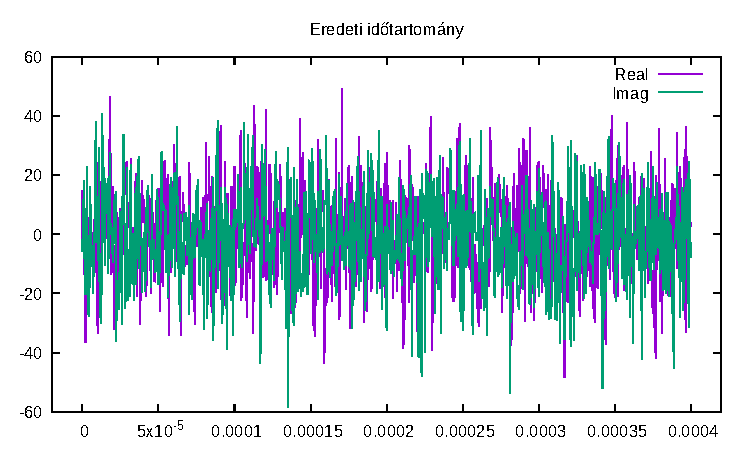
\includegraphics[width=\textwidth]{kep/original_samples.pdf}
			\subcaption{Az eredeti időtartománybeli jel első $1/512$-ed része (\qty{0.4}{ms}).}
		\end{subfigure}
		\begin{subfigure}{0.98\textwidth}
			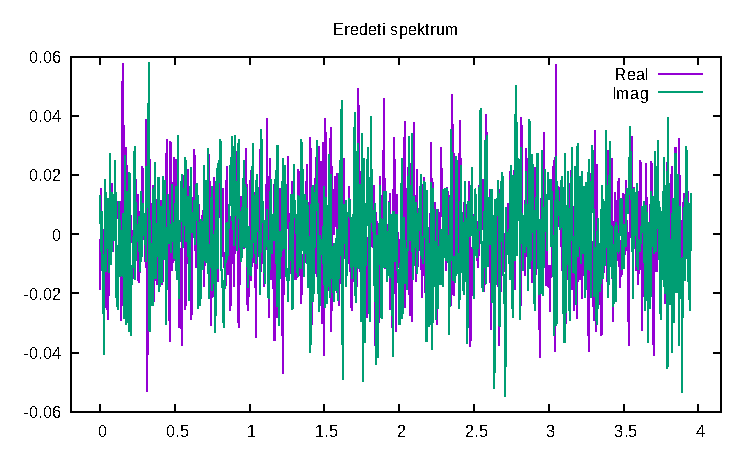
\includegraphics[width=\textwidth]{kep/original_spectrum.pdf}
			\subcaption{Az eredeti jel spektruma.}
		\end{subfigure}
		\caption{Az eredeti jel.}
		\label{fig:original}
	\end{figure}
	\subsection{Keverés}
		A diszkrét időtartománybeli komplex mintasorozat keverése egy komplex körforgó vektorral való szorzással lehetséges. Ehhez ki kell számolni, hogy milyen $\Delta\varphi$ szöggel kell elfordulnia a keverő vektornak mintánként.
		\begin{equation}
			b[i] = a[i]\cdot \exp(-j\cdot i\cdot\Delta\varphi)
		\end{equation}
		A keveréssel az $f_v$ komplex vivőfrekvenciáról keverek 0 frekvenciára, így
		\begin{equation}
			\exp(j\cdot i\cdot2\pi\dfrac{f_v}{f_s})\times\exp(-j\cdot i\cdot\Delta\varphi) = 1
		\end{equation}
		\begin{equation}
			\Delta\varphi = 2\pi\dfrac{f_v}{f_s}
		\end{equation}
		A keverés után jellegre változatlan mind az időtartománybeli jel ($a[i]$), mind a spektruma ($A[i]$), de valójában az egész spektrum eltolódott balra \qty{1.44}{MHz}-cel. Ez az eltolódás azért nem látszik az ábrákon, mert nem minden mintát plotolok ki, hanem csak minden 1024-ediket, hogy kicsi maradjon a fájlméret. Az időtartománybeli jeleknél viszont inkább csak a teljes időintervallum első 1/1000-edére ábrázolok, de azon belül minden mintát.
		\begin{figure}[h!]
			\centering
			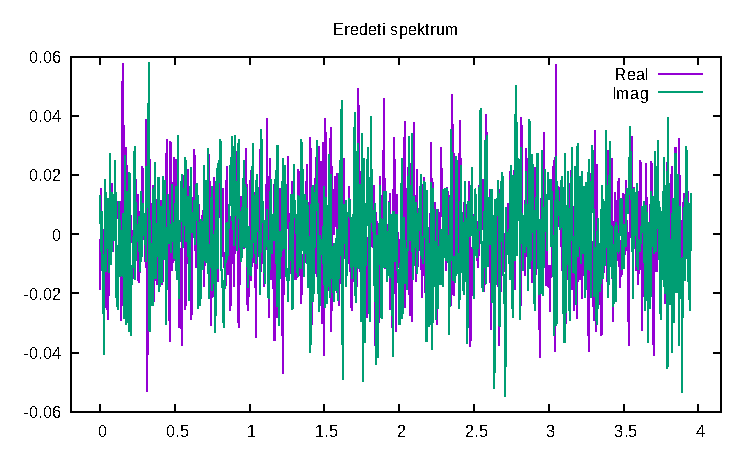
\includegraphics[width=0.98\textwidth]{kep/original_spectrum.pdf}
			\caption{Az keverés utáni jel spektruma.}
			\label{fig:mixed}
		\end{figure}
	\subsection{Aluláteresztő szűrés}
		Az én vivőmhöz tartozó jel feltehetőleg az $f_v\pm \dfrac{\Delta f_v}{2}$ sávon belül van, így a kevert jel spektrumának ($B[i]$) \qty{-40}{kHz} alatti és \qty{40}{kHz} feletti részét kinullázva, majd ezt vissza Fourier-transzformálva egy aluláteresztő-szűrt jelet lehet kapni ($c[i]$). Ehhez csak azt kell meghatározni, hogy a diszkrét spektrum melyik indexei között kell nullázni. A diszkrét spektrumban egy frekvencia-bin szélessége:
		\begin{equation}
			B_{bin} = \dfrac{f_s}{N}
		\end{equation}
		Ahol $N$ a minták száma. Tehát a kezdeti index ($k$) és végső index ($v$), ahol nullázni kell:
		\begin{align}
			k & = \dfrac{\qty{40}{kHz}\cdot N}{f_s} \\
			v & = N-k
		\end{align}
		\begin{figure}[h!]
			\centering
			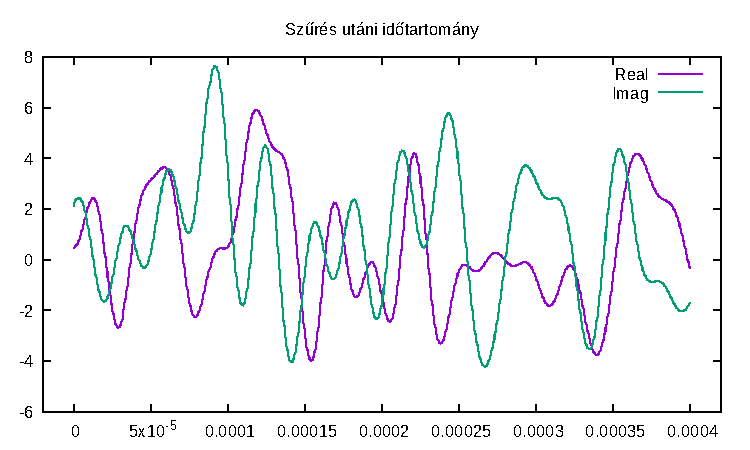
\includegraphics[width=\textwidth]{kep/filtered_samples.pdf}
			\caption{A szűrt időtartománybeli jel ($c[i]$) első $1/512$-ed része (\qty{0.4}{ms}).}
		\end{figure}	
		\begin{figure}[h!]
			\centering
			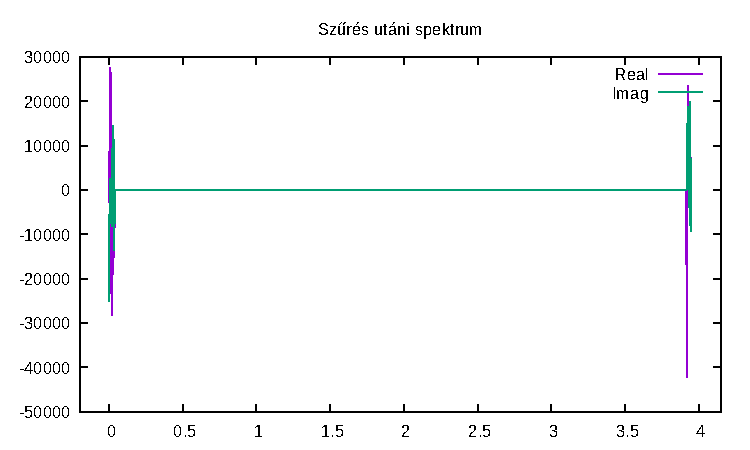
\includegraphics[width=\textwidth]{kep/filtered_spectrum.pdf}
			\caption{A szűrt jel spektruma ($C[i]$).}
		\end{figure}
	\subsection{Decimálás}
		A decimálást úgy végeztem el, hogy meghatároztam a decimálás $F$ faktorát, majd $F$ db szűrt minta  ($c[i]$) átlagát vettem egy mintának a decimált jelben ($d[i]$).
		\begin{equation}
			d[i] = \dfrac{1}{F}\sum_{l=(F-1)\cdot i}^{F\cdot i}c[l]
		\end{equation}
		A faktor egyszerűen a következőképpen adódik:
		\begin{equation}
			F = \dfrac{f_s}{f_{df}} = 100
		\end{equation}
	\subsection{Korrelálás}
		A kód számjegyeinek a sorozatából a hozzájuk tartozó QPSK szimbólumok konjugáltjait rendelte, majd ezzel egy csúszóablakos szorzatösszeg-számítással kaptam a korrelációt. \Aref{fig:correlated}. ábrán jól láthatóak a tüskék, amelyek egy a jelben lévő kódsorozat végét jelentik. \Aref{fig:megfejtes}. ábrán bejelöltem a szimbólumok határait piros vonalakkal, valamint a leolvasott biteket. A kezdeti szinkronizáló bitsorozatból az derül ki, hogy a Q csatorna negatív csúcsa felel meg az 1-es bitnek, a pozitív csúcsa pedig a 0-s bitnek.
		\begin{figure}[h!]
			\centering
			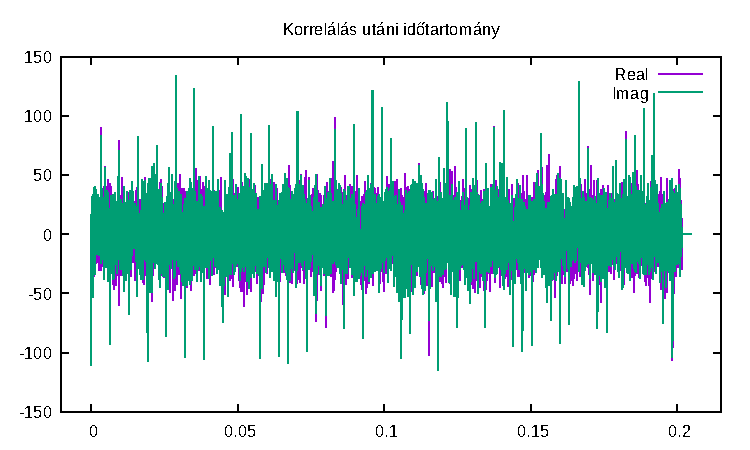
\includegraphics[width=0.98\textwidth]{kep/correlated_samples.pdf}
			\caption{A szórókóddal vett korreláció.}
			\label{fig:correlated}
		\end{figure}
		\begin{figure}[h!]
			\centering
			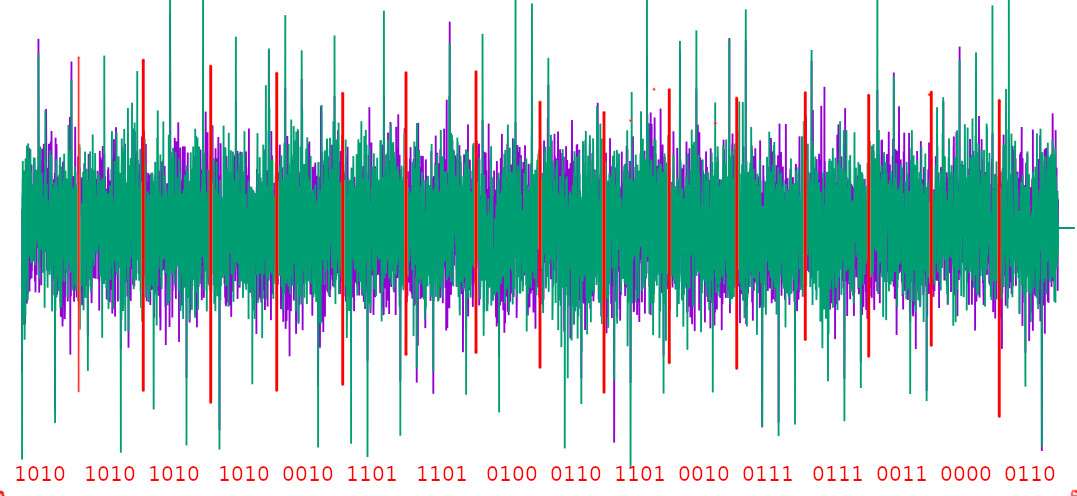
\includegraphics[width=0.98\textwidth]{kep/megfejtes.jpg}
			\caption{A megfejtés leolvasása.}
			\label{fig:megfejtes}
		\end{figure}

		Tehát a megfejtés szinkronizáló minta utáni része a következő: \verb|0x46D277306|
\bibliography{mybib}
\bibliographystyle{plain}
%
\clearpage
\appendix
%
\section{digitkf.h}
		\lstinputlisting{../c/src/digitkf.h}
\section{digitkf.c}
		\lstinputlisting{../c/src/digitkf.c}
\section{main.c}
		\lstinputlisting{../c/src/main.c}
%
\end{document}

%\cite{Henneron14}

%            \begin{align}
%                \label{equ:svd}
%                {\bf S}~=&~{\bf U \Sigma \adj{V}}
%            \end{align}

%            \begin{figure}
%                \centering
%                \includegraphics[width=0.8\textwidth]{kep/szerkesztett/wstk-mighty-gecko-nagy.jpg}
%                \caption{WSTK + radio board.}
%                \label{fig:wstkmighty}
%            \end{figure}
% \cite{Anritsu}
%            \begin{figure}
%                \centering
%                \begin{subfigure}{0.48\textwidth}
%                    \includegraphics[width=\textwidth]{kep/szerkesztett/sol-868-conducted.png}
%                    \caption{\SI{868}{MHz}}
%                \end{subfigure}
%                \begin{subfigure}{0.48\textwidth}
%                    \includegraphics[width=\textwidth]{kep/szerkesztett/sol-470-conducted.png}
%                    \caption{\SI{470}{MHz}}
%                \end{subfigure}
%                \caption{470 és \SI{868}{MHz}-es Sol radio board-ok kimeneti spektruma.}
%                \label{fig:sol-conducted}
%            \end{figure}

